
\section{Definition}

A second problem is the following,

Let $V = \left\{{v_1 , \cdots , v_n }\right\}$ be a set equipped with an unknown linear order. Given a subset of the relations $v_i \leq v_j$, determine the complete linear order by queries of the form: ``is $v_i \leq v_j$ ?''. (\cite{cardinal2013sorting})


\begin{figure}
	\centering
	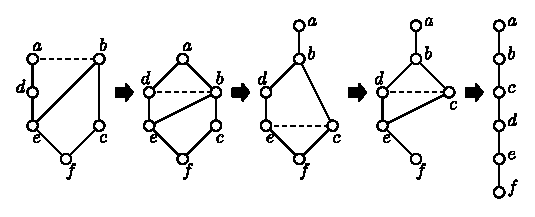
\includegraphics[width=0.7\textwidth]{fig/supi/ex1}
	\caption{\label{fig:supi/ex1} An instance of the problem of sorting under partial information. In this example, we use 4 comparisons (dashed edges). At every step, the Hasse diagram of the currently known partial order is shown. (\cite{cardinal2013sorting})}
\end{figure}


\section{History}

First appearance of the problem in \cite{fredman1976good} where an algorithm making $\BigO{\log e(P) + 2n}$ was featured. However this algorithm was not matching the ITLB for sub-linear $\log e(P)$. (\cite{cardinal2013sorting})

At that time, it remained open whether there existed, on the one hand, an algorithm performing $\BigO{\log e(P)}$ comparisons, and, on the other hand, an algorithm running in polynomial time. (\cite{cardinal2013sorting})

The first question was answered by \cite{kahn1984balancing}. They showed that there always exists a query of the form ``is $v_i \leq v_j$ ?'' such that the fraction of linear extensions in which $v_i$ is smaller than $v_j$ lies in the interval $(\sfrac{3}{11}, \sfrac{8}{11})$. This is a relaxation of the well-known $\sfrac{1}{3}$--$\sfrac{2}{3}$ conjecture, a conjecture formulated independently by Fredman, Linial, and Stanley, see \cite{linial1984information}. A simpler proof yielding weaker bounds was given by \cite{kahn1991balancing}. Better bounds were later given by \cite{brightwell1995balancing}, and \cite{brightwell1999balanced}. Iteratively choosing such a comparison yields an algorithm that performs $\BigO{\log e(P)}$ comparisons. However, finding the right comparisons in polynomial time remained intractable. (\cite{cardinal2013sorting})




\section{Algorithms}


The second question was anwered yes when the first polynomial-time algorithm achieving the bound $\BigO{\log e(P)}$ up to a constant factor was given by \cite{kahnkim1}. But due to the use of the ellipsoid algorithm, a costly optimization method, for choosing the right comparisons to make it could be considered inpractical.

Finally, in \cite{cardinal2013sorting}, new methods are developed. Three new algorithms having the same canvas : a first poly-time preprocessing phase followed by a $\BigO{\log e(P)}$ query phase. Caution has to be made though : each of the three different algorithms match the ITLB for a subset of the problem instances.

\begin{table}
	\begin{center}
	\caption{We denote by $E A(n)$ the time needed for the ellipsoid algorithm to compute the entropy of a poset of order $n$. The original bound given by \cite{kahnkim1} on the number of comparisons performed by their algorithm is $54.45 \cdot \log e(P)$. The improved bound given in the table is a byproduct of the results of \cite{cardinal2013sorting}. (The notation $\BigOe{n}$ means that the hidden constant may depend on $\epsilon$.) (\cite{cardinal2013sorting})}
	\label{tree:supi:table/jcardin}
	\begin{tabular}{|c|c|c|}

	\hline
	Algorithm & Global Complexity & Number of comparisons\\\hline\hline
	\cite{kahnkim1} & $\BigO{n \log n \cdot E A(n)}$ & $\leq 9.82 \cdot \log e(P)$\\\hline\hline
	\cite{cardinal2013sorting} \textbf{1} & $ \BigO{n^{2}} $ & $\BigO{\log n \cdot \log e(P)}$ \\\hline
	\cite{cardinal2013sorting} \textbf{2} & $ \BigO{n^{2.5}} $ & $\leq (1 + \epsilon) \log e(P) + \BigOe{n}$ \\\hline
	\cite{cardinal2013sorting} \textbf{3} & $ \BigO{n^{2.5}} $ & $\leq 15.09 \cdot \log e(P)$ \\\hline

	\end{tabular}
	\end{center}
\end{table}


\ref{tree:supi:table/jcardin} highlights the properties of the different algorithms, i.e.

\begin{itemize}

\item If $\log e(P)$ is super-linear in $n$, the number of comparisons of \cite{cardinal2013sorting} \textbf{2} is lower than that of \cite{kahnkim1}. By optimizing over $\epsilon$, it can be shown that the number of comparisons is actually $\log e(P) + \SmallO{\log e(P)} + \BigO{n}$ in this case, a number of comparisons comparable to that of Fredman’s algorithm.

\item If $\log e(P)$ is linear or sub-linear in $n$, the number of comparisons of \cite{cardinal2013sorting} \textbf{3} is comparable to that of \cite{kahnkim1}, although the constant in front of $\log e(P)$ is still far from the best constant achieved by a super-polynomial algorithm via balancing pairs \cite{brightwell1995balancing, brightwell1999balanced}.

\item Algorithms from \cite{cardinal2013sorting} have the following useful property: they compute information that guides the sorting and can then be reused to solve any given instance with the same partial information $P$, in time proportional to the number of comparisons, plus a term linear in $n$.

\end{itemize}


Looking at \ref{fig:supi/alg2}, algorithm 2 very much ressembles to what is done in \cite{jcardin1} for the Partial Order Production problem if we swap the roles of chains and antichains. This is explained in detail in \cite{DBLP:conf/birthday/CardinalF13}.


\begin{figure}
	\centering
	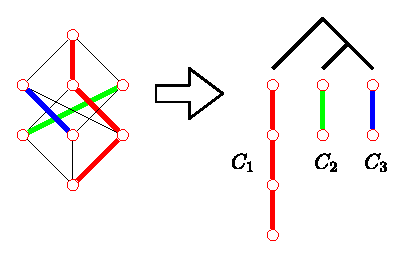
\includegraphics[width=0.7\textwidth]{fig/supi/alg2}
	\caption{\label{fig:supi/alg2} Illustration of algorithm 2. (\cite{cardinal2013sorting})}
\end{figure}



Indeed, Sorting Under Partial Information is the complement of Partial Order Production seen in \ref{tree:pop}.

\begin{align*}
& \concept{ITLB}(\text{partial order production}) + \concept{ITLB}(\text{sorting under partial information}) \\
&= \log(n!) - \log(e(P)) + \log(e(P)) \\
&= \log(n!) \\
&= \concept{ITLB}(\text{sorting})
\label{eq:complementarity}
\end{align*}